\section{Design}\label{sec:design}
In this chapter, I am going to describe all high-level technical details realized during the implementation of the demonstrator. Section \ref{subsec:examples} describes all the examples that I have conceptualized before choosing the final one for the implementation. This is then followed by the description of the steps taken for selecting the bx-tool in Section \ref{subsec:bxtoolselection}. Afterwards, Section \ref{subsec:architecturedesign} deals with the decisions taken for finalizing the apllication's architecture design.
\subsection{Choosing an Example}\label{subsec:exampleforimplementation}
To solve the problems as described in Section \ref{subsec:problem}, the main idea is to design and implement an interactive bx tool demonstrator based on an intuitive example.
\subsubsection{Construction}\label{subsubsec:exampleconstruction}
I have constructed a few examples for implementation as follows:
\paragraph{Task Management} This prototype can be used for allocating tasks in a team. It contains two views e.g., supervisor's view and employee's view. A Supervisor can allocate tasks to their subordinates. An employee can view the tasks assigned to him. Then the task will go through a life cycle as the work progresses, i.e., Assigned, In Progress, Testing, Done. Supervisor's view shows aggregate information from multiple projects and multiple employees, but does not contain detailed information, e.g., tasks have fewer states than for assigned employees. Bx rules control how updates are handled and states are reflected in the different views of the project, e.g., the employee's view will be updated for each state change, whereas the supervisor's view is only updated when a task is completed and not for intermediate changes.

\paragraph{Quiz} This prototype can be used for an online quiz game. It contains two views e.g., administrator's view and participant's view.
There will be a large set of questions related to different areas, e.g, history, geography, politics, sports, etc. The administrator can select the areas from which the questions will be shown to the participant and initiate the game. The participant can override the selection of the areas and start the quiz. Randomly questions will be shown to the participant from the selected areas with 4 options. The administrator's view contains less information than the participant's view, e.g., only the result of each question will be shown to the administrator, whereas participant can see questions along with its options. As soon as the participant chooses the answer to any question, bx rules control how updates are handled and states are reflected in the different views of the project.

\paragraph{Playing with Shapes} It contains two views e.g., low-level view (depicts \ac{UI} for low-level language, i.e., UI with less functionality) and high-level view (depicts UI for high-level language, i.e., UI with more functionality). User will draw a geometric shape, i.e., triangle / square / rectangle / circle with some notations similar to the shape on the low-level view and if the notations are correct, the high-level view tries to recognize the shape and draws it with default parameters and vice-versa. Basically the transformation will happen between a low-level language and a high-level language and bx rules control how updates are handled and states are reflected in the different views of the project. In high-level view, more functionalities will be present, i.e., moving one shape from one place to another, creating a clone of an existing shape, etc. which is not possible in low-level view.

\paragraph{Arranging a Kitchen}
It contains two views e.g., low-level view (depicts a grid structure containing blocks) and high-level view (empty space which depicts UI for kitchen). High-level view has more functionalities such as creating/ deleting/ moving an kitchen item, etc. out of which only a few will be available in low-level view. User will create/ delete/ move a kitchen item, i.e., sink / table on the high-level view and if changes done on the high-level view are according to the rules defined in the bx tool then items will be reflected on the low-level view with same colored blocks and vice-versa. Basically the transformation will happen between a low-level language and a high-level language and bx rules control how updates are handled and states are reflected in the different views of the project.

\paragraph{Person and Family}
It contains two views e.g., Family view and Person view. In Family view, it contains many families and each family consist of members. Whereas, Person view contains persons (the members of each family). We assume that the surnames are unique and allow us to differentiate between different families. Addition of a new person to the Person view will be reflected on the family view and vice-versa. Also, due to the uniqueness of the surnames, person created will be automatically assigned to the related family. Bx rules control how updates are handled and states are reflected in the different views.

\subsubsection{Selection}\label{subsubsec:exampleselection}
Selecting an example to implement through the demonstrator was not random, rather I have taken many factors into considerations before choosing the final one. It was a very important decision, as selection of the example and its implemenation will directly effect the research questions \textbf{\textit{RQ2}}, \textbf{\textit{RQ4.2}}, \textbf{\textit{RQ6}} described in Section \ref{subsec:approach} and requirements \textbf{\textit{NREQ2}}, \textbf{\textit{NREQ3}} described in Section \ref{subsec:functionalreq}.
\newline\newline Hence by taking into account all these factors, I have finally chosen the \textbf{Arranging a Kitchen} example to be implemented by the demonstrator as a part of my research. Following were the driving factors for the selection of the example:
\begin{itemize}
	\item {Any user can relate to the example very well as everybody is familiar with a kitchen and its environment.}
	\item {Example is very simple and no technical details are involved.}
	\item {Interactivity and rules won't be a overhead for the user, rather intuitive.}
	\item {Associted scenarios are part of day to day life, so user will be able to relate to the learning concepts through the example.}
\end{itemize}

\subsection{BX Tool Selection}\label{subsec:bxtoolselection}
Next step in the design process was selection of a bx tool which takes care of the bx part of the demonstrator and upon which the entire framework of the demonstrator will be constructed. My gathered information during the case study phase led the foundation for the selection process.
\subsubsection{Theory}\label{subsubsec:bxtooltheory}
I further investigated on the existing bx tools from the point of view of practical application and usage of these tools in terms of building softwares. Even after a significant amount of work has been done by developers community and bx community, the main problems are still revolving around below points \cite{bx-theoryandappl}: 
\begin{itemize}
	\item {the conceptual or theoretical challenges, practical challenges associated with using bx, and tool/technology challenges involved with building software systems that supported or exploited bx.}
	\item {limited benchmarks for comparison of complete bx solutions.}
	\item {no common repository of bx scenarios or problems that can be used to test and evaluate bx solutions.}
	\item {there exists tools to support particular bx scenarios but with very limited interoperability and integration.}
\end{itemize}
To focus particularly on the above issues, bx-community had conducted a series of technical workshops at relevant conferences and organised week-long intensive research seminars in the year 2013 before the \textit{BX 2014} workshop \cite{bx-theoryandappl}. Some of the main outcome of these seminars are listed below:
\begin{itemize}
	\item {focus on the need of benchmarks and further categorizing them into functional and non-functional ones.}
	\item {scenarios for bx were developed based on database, synchronization, model-view architecture etc.}
	\item {software tool support for bx was shown in terms of demos which includes tool like eMoflon, Echo etc.}
\end{itemize}
\subsubsection{Selection}\label{subsubsec:bxtoolselection}
Again, it was a very important decision, as selection of the bx tool and the implemenation on the top of it will directly effect the research questions \textbf{\textit{RQ1}}, \textbf{\textit{RQ4.1}} described in Section \ref{subsec:approach} and requirements \textbf{\textit{NREQ1}} described in Section \ref{subsec:functionalreq}.
\newline\newline The outcome of the seminars as discussed in previous section \ref{subsubsec:bxtooltheory} led me to concentrate and analyze the bx tools like eMoflon, Echo, BIGUL. Also, I came across the benchmark \cite{benchmarx} \cite{benchmarx-reload}, the first non-trivial benchmark where Anjorin et al. has provided a practical framework to compare and evaluate three bx tools. After analyzing these tools, benchmarks and taking into consideration the reserach questions and requiements, I have finally chosen \textbf{eMoflon} as the bx tool to handle the bx part of my demonstrator. Following were the driving factors for the selection of the bx tool:
\begin{itemize}
	\item {sample implementation with framework to implement the eMoflon tool was already available.}
	\item {my supervisor/prof. is a core member of the eMoflon community which gave me added advantage of knowing the tool inside out.}
	\item {extra knowledge about the tool can be really handy and it actually helped me in solving the implemenation issues/challenges regarding the tool as described in Section\ref{subsec:implchallenges}.}
\end{itemize}

\subsubsection{Benchmarx}\label{subsubsec:benchmarx}
A bx benchmark (referred to as \textbf{Benchmarx} from now on) is a bx example that has a precise and executable definition of a binary consistency relation on source and target artefacts; an explicit definition of, or a generator for, input artefact elements; a set of precisely defined update scenarios for certain input artefact elements; and a set of executable metric definitions \cite{bx-theoryandappl}.
\newline\newline Anjorin et al. \cite{benchmarx-reload} tried to solve the main problem with benchmarking bx tools by creating a common design space, in which different bx tools architecture can be accomodated irrespective of the fact that they can have different input data. 
\paragraph{Design Space} 

\subsection{Architecture Design}\label{subsec:architecturedesign}
Last step in the design process was application architecture design which is the most important part of my thesis and also the starting phase of the implementation of the prototype.
\subsubsection{Design Decision}\label{subsubsec:architecturedesigndecision}

\subsubsection{Framework}\label{subsubsec:framework}
Figure~\ref{fig:Architecture_Diagram} shows a very high-level architecture diagram of my prototype. It consist of 3 layers e.g., View, Controller and Model. View is responsible for all the graphical user interface management and consist of technologies like HTML, CSS, JavaScript and Jquery. Controller is responsible for event handling and basically consist of the technology Servlet. Model is responsible for all the tasks related to business logic, business rules, data, meta-models, state of meta-models etc. and consist of java classes.
\begin{figure}
	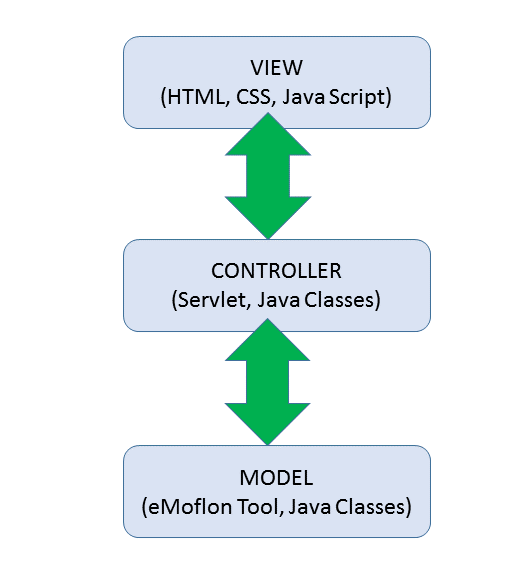
\includegraphics[width=1\textwidth]{figures/Highlevel_Arch}
	\caption{High Level Architecture Diagram}
	\label{fig:Architecture_Diagram}
\end{figure}
\clearpage
\paragraph{Request-Response Cycle} 
Figure~\ref{fig:Architecture_Diagram} shows a detailed architecture diagram with a complete request-response cycle.
\begin{figure}
	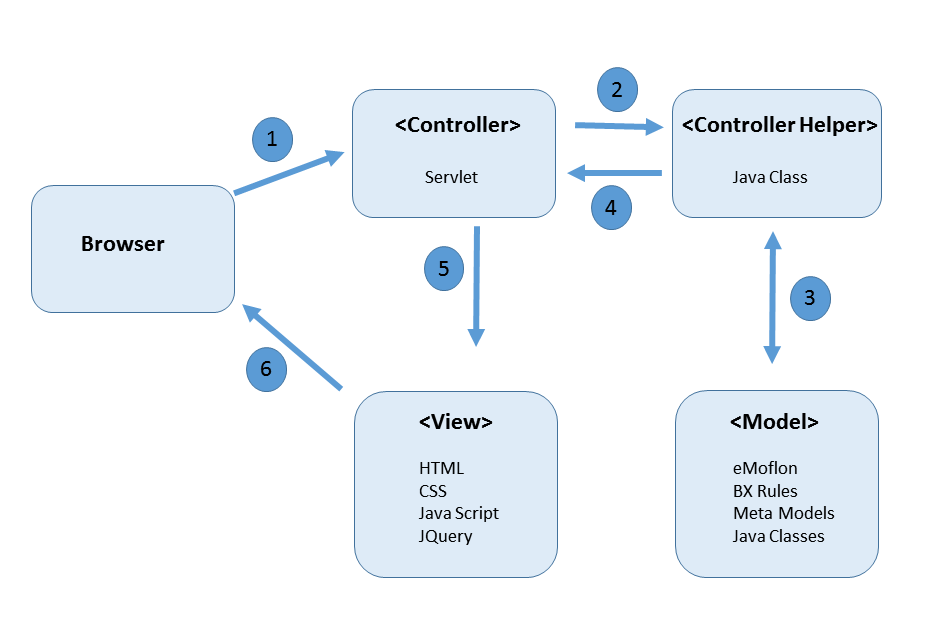
\includegraphics[width=1\textwidth]{figures/Detail_Arch}
	\caption{Detail Architecture Diagram}
	\label{fig:Detail_Architecture_Diagram}
\end{figure}

\subsubsection{Controller}\label{subsubsec:controller}

\subsubsection{Model}\label{subsubsec:model}
\paragraph{UI Models}
\paragraph{Kitchen Layout}
\paragraph{Grid Layout}

\subsubsection{View}\label{subsubsec:view}
\paragraph{External Design}
\paragraph{Internal Design}

\subsection{Challenges}\label{subsec:designchallenges}
architecture design issues- dependencies of projects 

UI design - high level/low level views, deltas, low level view user interaction(color), user interaction

\subsection{Walkthrough}\label{subsec:walkthrough}






